\section{预训练}
与 GLM-4.5 类似，GLM-5 的基座模型经历两个阶段：用于通用语言与编码能力的预训练，以及用于智能体与长上下文能力的中期训练。我们扩展了 GLM-5 各训练阶段的 token 预算，基座模型总计使用 28.5 万亿 tokens。

\subsection{架构}

\paragraph{模型规模扩展。} GLM-5 将专家数扩展到 256，并将层数降至 80，以降低专家并行通信开销。由此得到 744B 参数模型（40B 激活参数），相较 GLM-4.5（355B 总参数、32B 激活参数）在总规模上翻倍。

\begin{table}[!ht]
    \small
    \centering
    \caption{GQA-8 与 MLA 各变体的评测结果。}
    \begin{tabular}{c|cccccccc}
        \toprule
        Dataset & Hellaswag & MMLU & C-Eval & RACE & BBH & GSM8K & HumanEval \\
        \midrule
        GQA-8 & 77.3 & 61.2 & 60.0 & 79.6 & \textbf{53.3} & \textbf{47.6} & \textbf{38.5} \\
        MLA & 77.3 & 61.5 & 59.7 & 77.8 & 48.9 & 46.2 & 33.5 \\
        MLA + Muon Split & \textbf{77.8} & \textbf{62.5} & \textbf{62.1} & \textbf{79.9} & 51.8 & 45.0 & 36.7\\
        MLA-256 + Muon Split & 77.4 & 62.0 & 59.9 & 79.6 & 51.3 & 47.5 & 36.6 \\
        \bottomrule
    \end{tabular}
    \label{tab:mla}
\end{table}

\paragraph{多潜变量注意力。} 通过使用降维的 key-value 向量，Multi-latent attention（MLA）~\cite{liu2024deepseekv2} 能在效果上匹配 Grouped-Query Attention（GQA），同时在长上下文序列上带来更优的 GPU 显存节省与更快处理速度。

然而，在使用 Muon 优化器的实验中，我们发现采用 576 维潜变量 KV-cache 的 MLA 无法达到 8 组查询的 GQA（记作 GQA-8，2048 维 KV-cache）性能。为弥合该差距，我们对 GLM-4.5 的 Muon 配方进行改造。
在原始配方中，我们对多头查询、键、值的上投影矩阵 $W^{UQ}, W^{UK}, W^{UV}$ 施加矩阵正交化。我们改为将这些矩阵按不同头拆分为更小矩阵，并分别施加矩阵正交化。该方法记作 Muon Split，可使不同注意力头的投影权重以不同尺度更新。\Cref{tab:mla} 表明，该方法有效提升 MLA 性能并匹配 GQA-8。实践中我们还发现，在 Muon Split 下，GLM-5 在预训练期间的注意力 logits 尺度保持稳定，无需任何截断策略。

MLA 的另一个缺点是解码时计算成本较高。解码阶段，MLA 需要 576 维点积，高于 GQA 的 128 维计算。虽然 DeepSeek-V3 的注意力头数依据 H800 的 roofline 选取~\cite{zhao2025insights}，但这并不适用于其他硬件。考虑到 MLA 在训练与 prefilling 阶段呈现 Multi-head Attention（MHA）形态，我们将头维度由 192 提升到 256，并将注意力头数减少 1/3。在保持训练计算量
与参数量不变的前提下，这一改动降低了解码计算。该变体在 \Cref{tab:mla} 中记作 MLA-256，在 Muon Split 下与 MLA 性能相当。

\begin{wraptable}{r}{0.4\linewidth}
    \centering
    \caption{DeepSeek-V3.2 与 GLM-5 的接受长度对比。}
    \label{tab:mtp}
    \begin{tabular}{c|c}
        \toprule
        Model  & Accept Length \\
        \midrule
        DeepSeek-V3.2 & 2.55 \\
        GLM-5  & \textbf{2.76}\\
        \bottomrule
    \end{tabular}
\end{wraptable}

\paragraph{参数共享的多 token 预测。} Multi-token prediction（MTP）~\cite{gloeckle2024mtp,liu2024deepseek} 可提升基座模型性能，并可作为 speculative decoding~\cite{leviathan2023spec} 的草稿模型。然而训练时若要预测后续 $n$ 个 token，需要 $n$ 个 MTP 层。因此，MTP 参数与 kv cache 的显存占用会随投机步数线性增长。DeepSeek-V3 改为只训练单个 MTP 层，并在推理时预测后续 2 个 token，但训练-推理不一致会降低第二个 token 的接受率。为此，我们提出在训练时共享 3 个 MTP 层参数。这样可在与 DeepSeek-V3 一致的草稿模型内存成本下提升接受率。\Cref{tab:mtp} 显示，在我们私有提示集上、相同投机步数（4）条件下，GLM-5 的接受长度长于 DeepSeek-V3.2。

\subsubsection{使用 DeepSeek Sparse Attention（DSA）进行继续预训练}
\begin{table}[!ht]
    \centering
    \caption{MLA 与 DSA 基座模型在长上下文基准上的对比。}
    \begin{tabular}{c|cccc}
    \toprule
     & MQ-NIAH-128k & MV-NIAH-128k & SQuAD-128k & HotpotQA-128k \\
    \midrule
    MLA & \textbf{100.0} & 95.5 & 79.7 & \textbf{66.3} \\
    DSA & \textbf{100.0} & \textbf{97.0} & \textbf{86.0} & 63.0\\
    \bottomrule
    \end{tabular}
    \label{tab:dsa}
\end{table}
我们在训练中使用 DSA。
DSA~\cite{deepseekai2025deepseekv32pushingfrontieropen} 的核心思想，是用动态细粒度选择机制替代传统稠密 $O(L^2)$ 注意力——后者在 $128\text{K}$ 上下文下成本极高。不同于固定模式（如滑动窗口），DSA 会“查看”内容并决定哪些 token 重要。
从研究者视角看，DSA 的一个关键点在于它通过在稠密基座模型上进行继续预训练引入，避免了“天文级”从零训练成本。该迁移遵循“两阶段：稠密预热 + 稀疏训练适配”策略。DeepSeek-V3.2-Exp 在基准性能上保持与其稠密前代一致，证明长上下文中约 90\% 的注意力项确实冗余。
DSA 在长序列上可将注意力计算降低约 1.5-2×，这对我们构建的推理型智能体非常关键，使其可以在约一半 GPU 成本下处理 128K 上下文。

\begin{figure}
    \centering
    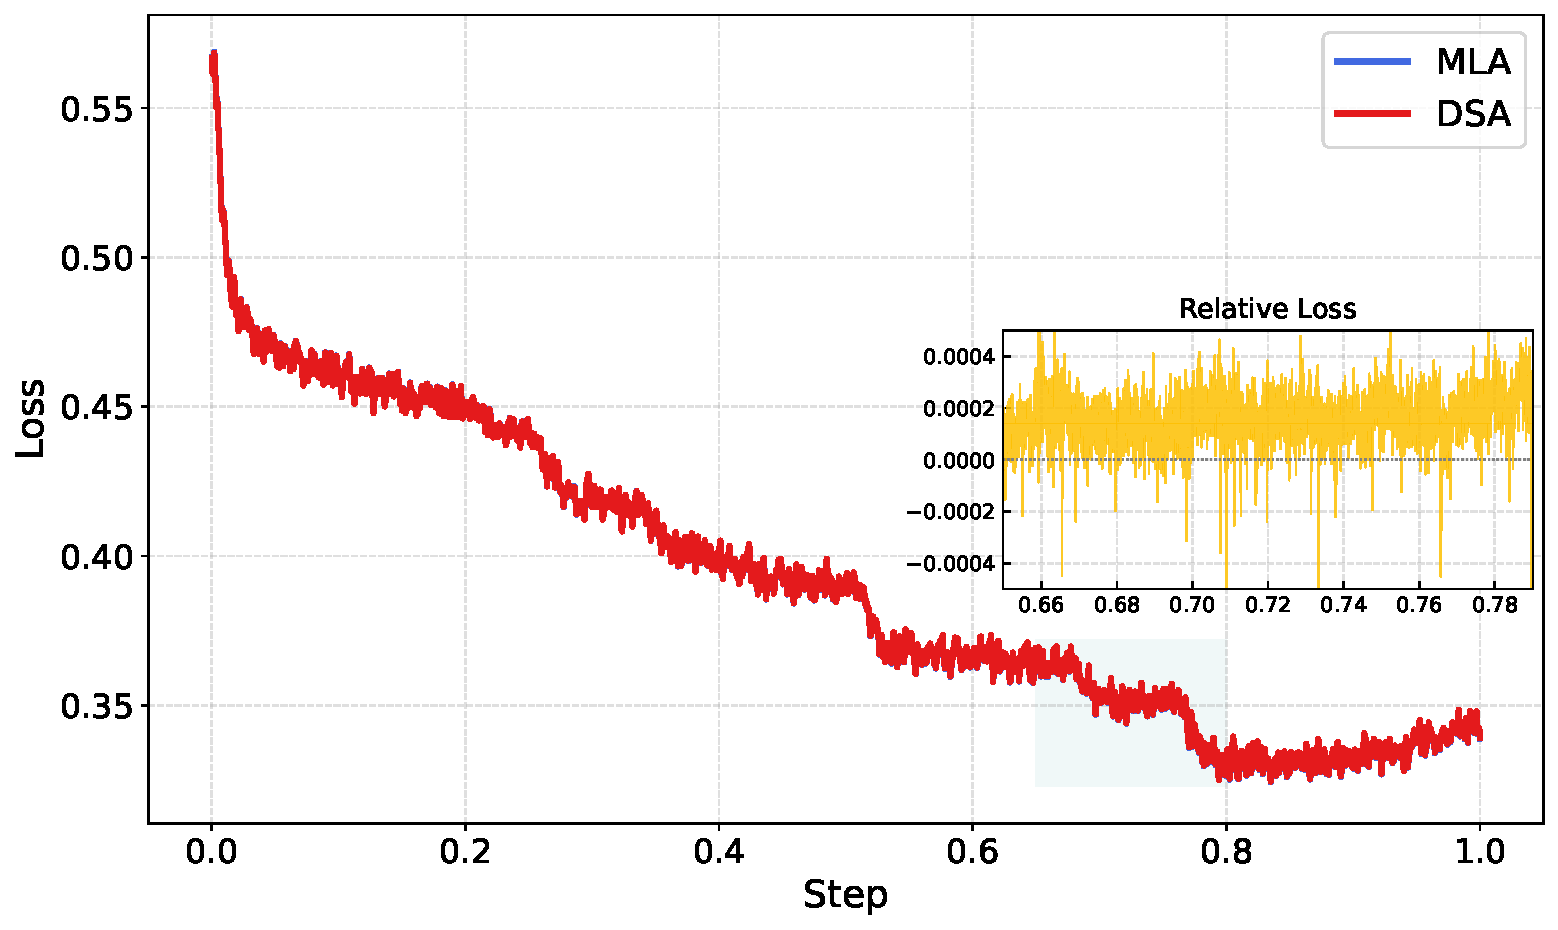
\includegraphics[width=0.6\linewidth]{figures/loss_v2.pdf}
    \caption{MLA 与 DSA 训练的 SFT loss 曲线对比。结果使用窗口大小为 50 的滑动平均进行平滑。}
    \label{fig:placeholder}
\end{figure}

DSA 训练从中期训练结束时的基座模型启动。预热阶段进行 1000 步，每步使用 14 条长度 202,752 tokens 的序列，最大学习率为 5e-3。随后稀疏适配阶段沿用中期训练的数据与超参，训练 20B tokens。尽管训练预算远小于 DeepSeek-V3.2（943.7B tokens），我们发现这已足以将 DSA 模型适配到与原 MLA 模型相当的性能。\Cref{tab:dsa} 显示，DSA 模型的长上下文性能与 MLA 模型接近。为进一步验证 DSA 训练有效性，我们分别使用相同 SFT 数据微调 DSA 与 MLA 模型，发现两者在训练 loss 与评测基准上持平。

\subsubsection{高效注意力变体的消融研究}

除 DSA~\cite{liu2025deepseek} 外，我们基于 GLM-9B\footnote{我们 GLM-4 系列模型之一，见 https://github.com/zai-org/GLM-4} 探索了多种替代性高效注意力机制。基线在全部 40 层使用 group query attention，并已在 128K 上下文窗口上完成微调。我们评测以下方法：

\begin{itemize}[leftmargin=1.5em,itemsep=2pt]
    \item {{Sliding Window Attention（SWA）Interleave：}} 在网络中统一应用全注意力层与窗口注意力层固定交替模式。
    \item {{Gated DeltaNet（GDN)}~\cite{yanggated}：} 一种线性注意力变体，以门控线性递推替代二次复杂度的 softmax 注意力计算，将注意力计算成本从序列长度的二次降为线性。
\end{itemize}

\noindent 基于这些基线，我们提出两项改进：

\begin{itemize}[leftmargin=1.5em,itemsep=2pt]
    \item {SWA Pattern（基于搜索）：} 受 PostNAS~\cite{gu2025jet} 启发，我们提出基于搜索的适配方法，识别最优层子集进行 SWA 转换，并在其余层保留全注意力。我们使用 beam search，在长上下文下游任务上最大化性能。为降低计算成本，我们仅在 16K 上下文长度进行搜索，并将所得模式泛化到其他长度。具体而言，beam size 设为 8，每步优化两层；对于 40 层的 GLM-9B，约 10 步收敛。每步在 16K 的 RULER 基准~\cite{hsiehruler} 上评估候选模式，并保留前 8 个候选进入下一步。最终模式为 \texttt{SFSSFFSSSFFFFSSFSFFFFFFSFSFSSFSSFSFSSFSSS}，其中 \texttt{S} 与 \texttt{F} 分别表示 SWA 与全注意力层。表~\ref{tab:ruler_results} 显示，该搜索配置显著优于固定交替方式。值得注意的是，尽管仅在 16K 优化，该模式在长度泛化上表现稳健，在所有测试长度上都保持有效。

    \item {SimpleGDN：} 一种极简线性化策略，旨在最大化复用预训练权重，改进 GDN 在继续训练适配中的表现。我们完全移除 \texttt{Conv1d} 与显式门控模块，转而将预训练的 Query、Key、Value 投影权重直接映射到线性递推形式。该简化在保留线性注意力效率收益的同时，消除了额外参数需求。
\end{itemize}

\begin{table}[h]
    \small
    \centering
    \caption{GLM-9B 基线与两种 SWA 变体在 \emph{不进行任何额外训练} 条件下的 RULER 结果。两种 SWA 都采用 1:1 的全注意力层与 SWA 层比例，窗口大小 4096。基于搜索的 SWA 模式仅在 16k 上发现一次，并统一应用于所有输入长度。}
    \label{tab:ruler_results}
    \begin{tabular}{lcccccc}
        \toprule
         & {4K} & {8K} & {16K} & {32K} & {64K} & {128K} \\
        \midrule
        GLM-9B (Full Attn)  & 95.19 & \textbf{93.67} & \textbf{92.01} & \textbf{91.09} & \textbf{85.35} & \textbf{75.28} \\
        SWA Interleave      & 94.87 & 54.02 & 25.89 & 12.61 &  8.32 &  6.51 \\
        SWA Pattern & \textbf{95.78} & 92.54 & 88.92 & 82.52 & 70.23 & 53.95 \\
        \bottomrule
    \end{tabular}
\end{table}

我们在四个长上下文基准上评测所有方法：RULER~\cite{hsiehruler}、MRCR\footnote{\url{https://huggingface.co/datasets/openai/mrcr}}、HELMET-ICL~\cite{yen2024helmet} 和 RepoQA~\cite{liu2024repoqa}。结果见表~\ref{tab:gqa_results_appendix}。我们在 64K 上下文长度下对每种方法继续训练 190B tokens，并保持高效注意力层与全注意力层 1:1 比例。对于 GDN 和 SimpleGDN，我们遵循 Jet-Nemotron~\cite{gu2025jet} 流程。

\begin{table*}[h]
\centering
\caption{长上下文基准结果。所有高效注意力变体均从 GLM-9B 全注意力基线继续训练而来。SWA pattern 表示基于搜索的层选择；SWA interleave 表示固定交替模式。$\Delta$@64K 与 $\Delta$@128K 分别表示相对全注意力基线在 64K 和 128K 上下文下的差值。}
\label{tab:gqa_results_appendix}
\resizebox{\textwidth}{!}{
\begin{tabular}{lcccc}
\toprule
  & \textbf{RULER (64K\,/\,128K)}
  & \textbf{MRCR (64K\,/\,128K)}
  & \textbf{HELMET-ICL (64K\,/\,128K)}
  & \textbf{RepoQA (64K\,/\,128K)} \\
\midrule
GLM-9B 
  & 85.35\,/\,75.28
  & 36.53\,/\,35.39
  & 77.68\,/\,77.36
  & 69.00\,/\,65.83 \\
\midrule
SWA Interleave
  & 65.94\,/\,44.93 {\scriptsize($\downarrow$19.41\,/\,$\downarrow$30.35)}
  & 30.03\,/\,28.83 {\scriptsize($\downarrow$6.50\,/\,$\downarrow$6.56)}
  & 75.96\,/\,63.52 {\scriptsize($\downarrow$1.72\,/\,$\downarrow$13.84)}
  & 50.33\,/\,39.33 {\scriptsize($\downarrow$18.67\,/\,$\downarrow$26.50)} \\
SWA Pattern
  & \textbf{83.72\,/\,69.59} {\scriptsize($\downarrow$1.63\,/\,$\downarrow$5.69)}
  & \textbf{35.02\,/\,33.58} {\scriptsize($\downarrow$1.51\,/\,$\downarrow$1.81)}
  & 76.48\,/\,74.60 {\scriptsize($\downarrow$1.20\,/\,$\downarrow$2.76)}
  & 62.33\,/\,51.17 {\scriptsize($\downarrow$6.67\,/\,$\downarrow$14.66)} \\
GDN
  & 76.76\,/\,64.00 {\scriptsize($\downarrow$8.59\,/\,$\downarrow$11.28)}
  & 31.72\,/\,30.22 {\scriptsize($\downarrow$4.81\,/\,$\downarrow$5.17)}
  & 76.88\,/\,74.84 {\scriptsize($\downarrow$0.80\,/\,$\downarrow$2.52)}
  & 65.50\,/\,56.17 {\scriptsize($\downarrow$3.50\,/\,$\downarrow$9.66)} \\
SimpleGDN
  & 81.76\,/\,67.03 {\scriptsize($\downarrow$3.59\,/\,$\downarrow$8.25)}
  & 33.03\,/\,31.27 {\scriptsize($\downarrow$3.50\,/\,$\downarrow$4.12)}
  & \textbf{79.80\,/\,81.84} {\scriptsize($\uparrow$2.12\,/\,$\uparrow$4.48)}
  & \textbf{65.50\,/\,58.50} {\scriptsize($\downarrow$3.50\,/\,$\downarrow$7.33)} \\
\bottomrule
\end{tabular}
}
\end{table*}

表~\ref{tab:gqa_results_appendix} 显示了高效注意力方法间清晰的性能-效率权衡层级。朴素交替的滑动窗口注意力（SWA）在长上下文任务上会出现灾难性退化（例如 RULER@128K 下降 30.35），而基于搜索的层选择通过在关键层保留全注意力显著缩小了该差距。GDN 等线性注意力变体进一步提升质量，但需引入额外参数；SimpleGDN 通过最大化复用预训练权重取得了最佳平衡。尽管如此，这些方法在细粒度检索任务上仍存在固有精度差距——在 RULER@128K 上最多下降 5.69 分，在 RepoQA@128K 上最多下降 7.33 分——原因在于继续训练适配时高效注意力机制不可避免的信息损失，即便有一半层保留全注意力。相比之下，DSA 在构造上是无损的：其 lightning indexer 在不丢弃任何长程依赖的情况下实现 token 级稀疏，可应用于全部层且不引入质量退化。


为验证这一点，我们在采用多潜变量注意力的 GLM-4.7-Flash\footnote{\url{https://huggingface.co/zai-org/GLM-4.7-Flash}} 上开展了小规模 DSA 实验。按标准 DSA 配方，训练分两阶段：(i)~\textit{warmup} 阶段仅训练 indexer 1000 步（batch size 16），并冻结所有基座模型权重；随后 (ii)~\textit{joint-training} 阶段在 150B tokens 上联合训练模型与 indexer。
表~\ref{tab:dsa_ruler_results} 给出了 4K 到 128K 上下文长度下的 RULER 结果。仅 warmup 变体（\textit{GLM-4.7-Flash + DSA warmup}）已保留了基线的大部分性能；性能下降较小且主要集中在最长上下文窗口（128K: $79.21 \to 71.35$），短上下文几乎不受影响。完成 150B tokens 联合训练后，\textit{GLM-4.7-Flash + DSA} 几乎弥合了全部残余差距：在 16K（$+0.86$）、32K（$+0.49$）和 64K（$+1.72$）上\textit{超过}基线，而在 128K 仅落后 0.35 分。

\begin{table}[t]
    \small
    \centering
    \caption{GLM-4.7-Flash 使用 DSA 的 RULER 结果。
    仅 warmup 变体只训练 indexer，
    并保持基座模型冻结；完整 DSA 变体对二者联合训练
    150B tokens。 }
   \label{tab:dsa_ruler_results}
    \begin{tabular}{lcccccc}
        \toprule
         & {4K} & {8K} & {16K} & {32K} & {64K} & {128K} \\
        \midrule
        GLM-4.7-Flash  & 97.44 & 96.72 & 95.83 & 92.96 & 85.34 & 79.21 \\
        GLM-4.7-Flash + DSA warmup & 97.51 & 96.54 & 95.40 & 90.09 & 84.05 & 71.35  \\
        GLM-4.7-Flash + DSA & 96.77 & 96.25 & 96.69 & 93.45 & 87.06 & 78.86 \\
        \bottomrule
    \end{tabular}
\end{table}



\subsection{预训练数据}

\paragraph{Web。} 在 GLM-4.5 数据流水线基础上，我们优化了海量网页数据的筛选标准。我们引入了另一个基于句向量的 DCLM~\cite{li2025datacomplmsearchgenerationtraining} 分类器，用于识别并聚合标准分类器之外的高质量数据。为应对长尾知识问题，我们使用世界知识分类器（基于 Wikipedia 条目与 LLM 标注数据优化）从中低质量数据中提炼有价值信息。

\paragraph{代码。} 我们扩展了代码预训练语料，纳入主要代码托管平台更新快照和更大规模含代码网页，模糊去重后的唯一 token 增长 28\%。为提升语料完整性并降低噪声，我们修复了 Software Heritage 代码文件中的元数据对齐问题，并采用更准确的语言分类流程。我们延续 GLM-4.5 的质量感知采样策略，用于源码与代码相关网页文档。此外，我们还为更广泛的低资源编程语言（如 Scala、Swift、Lua 等）训练专用分类器，提升这些语言的采样质量。

\paragraph{数学 \& 科学。} 我们从网页、书籍与论文收集高质量数学与科学数据，以进一步增强推理能力。具体而言，我们改进了网页内容抽取流水线，以及书籍和论文的 PDF 解析机制，从而提升数据质量。我们使用大语言模型对候选文档打分，仅保留最具教育价值的内容。针对长上下文文档，我们开发了分块聚合打分算法以提升评分准确性。过滤流程严格避免使用合成、AI 生成或模板化数据。



\subsection{中期训练}

在 GLM-4.5 引入的中期训练框架基础上，我们在 GLM-5 中进一步扩大训练规模与最大上下文长度，以持续增强模型的推理、长上下文与智能体能力。

\paragraph{扩展上下文与训练规模。} 我们分三阶段渐进扩展上下文窗口：32K（1T tokens）、128K（500B tokens）和 200K（50B tokens）。相较 GLM-4.5 的 128K 上限，新增的 200K 阶段显著提升了模型处理超长文档和复杂多文件代码库的能力。在后续阶段，我们相应上采样长文档与合成智能体轨迹。

\paragraph{软件工程数据。} 我们保留了将仓库级代码文件、commit diff、GitHub issue、pull request 及相关源码拼接为统一训练序列的范式。在 GLM-5 中，我们放宽仓库级过滤标准以扩大可用仓库池，得到约 1000 万组 issue–PR 对；同时加强 issue 级质量过滤以降低噪声。我们还为每组 issue–PR 检索更大规模相关文件，获得更丰富的开发上下文与更广的真实软件工程场景覆盖。过滤后，issue–PR 部分数据约含 160B 唯一 tokens。

\paragraph{长上下文数据。} 我们的长上下文训练集由自然数据与合成数据构成。自然数据来自书籍、学术论文和通用预训练语料中的文档，并通过多阶段过滤（PPL、去重、长度）与知识密集领域上采样进行构建。受 NextLong\cite{gao2025nextlongeffectivelongcontexttraining} 与 EntropyLong\cite{jia2025entropylongeffectivelongcontexttraining} 启发，在合成数据构建中我们采用多种技术构造长程依赖。我们通过交错打包将高相似文本聚合为序列，以缓解 lost-in-the-middle 现象并提升多类长上下文任务性能。在 200K 阶段，我们额外引入少量类似 MRCR 的数据，并设计多个变体扩展 OpenAI 原始范式，以增强超长多轮对话中的召回。经验上我们发现，逐步增加数据多样性能持续提升模型长上下文性能；尤其是在初始 128K 阶段之上追加 200K 中期训练后，模型即便在 128K 窗口内的表现也进一步增强。

\subsection{训练基础设施}

\subsubsection{内存效率}

\textbf{灵活的 MTP 放置。} 在交错流水并行~\cite{narayanan2021efficientlargescalelanguagemodel} 下，模型组件可灵活分配到各 stage。MTP 模块横跨 embedding、transformer 与 output 组件，其内存占用显著高于其他模块，导致 stage 级不平衡。我们将 MTP 输出层与主输出层共置于最后一段以共享参数，同时将其 embedding 与 transformer 组件放在前一段。这样可降低最后一段内存压力并改善流水各 rank 的均衡性。

\textbf{Pipeline ZeRO2 梯度分片。} 每个 pipeline rank 包含多个 stage~\cite{narayanan2021efficientlargescalelanguagemodel}，朴素实现下每个 stage 都需完整梯度缓冲区用于累积与优化器更新。受 ZeRO2~\cite{rajbhandari2020zeromemoryoptimizationstraining} 启发，我们在数据并行维度对梯度进行分片，使每个 stage 仅存储完整梯度的 1/dp。另进一步，仅为两个 stage 保留完整累积缓冲，并通过双缓冲复用。当一个 stage 缓冲在连续 microbatch 上累积梯度时，前一 stage 缓冲的梯度同步并行进行。这将持久梯度内存降低为“每 stage 分片缓冲 + 两个完整滚动累积缓冲”，在实践中不增加额外同步开销。

\textbf{Muon 分布式优化器的零冗余通信。} 朴素 Muon 实现会在每个数据并行 rank 上 all-gather 全量模型参数，造成瞬时内存峰值和冗余通信。我们将 all-gather 限定为各 rank 持有的参数分片，并将本地计算与分片通信重叠。该方案消除了冗余通信，显著降低了优化器相关峰值内存开销。

\textbf{流水激活值卸载。} 在流水 warmup 期间，前向执行先于反向，导致中间激活值生存期拉长。我们在前向后将激活值卸载到主机内存，并在反向前重载~\cite{298555}。卸载按层粒度进行，进一步降低峰值内存。结合细粒度重计算后，基本无需将激活值常驻 GPU 显存。卸载与重载被调度为与计算重叠，同时避免与点对点通信及 MoE token 路由（dispatch 与 combination）争用。该方案在近零开销下显著降低激活值内存占用。

\textbf{序列分块输出投影以降低峰值内存。} 
输出投影与交叉熵损失在反向传播激活保存和损失计算精度提升时会产生瞬时内存开销。为降低该开销，我们将输入序列切分为更小块，对每块独立计算投影与损失，完成该块前后向并释放激活后再处理下一块。块数增加时，峰值内存随之下降。采用合适块数可在保持与不分块执行相近性能的同时，缓解输出层内存压力。


\subsubsection{并行效率}

\textbf{高效延迟权重梯度计算。} 为减少流水气泡，我们将关键路径上的部分权重梯度计算延后~\cite{qi2023zero}。结合优化后的存储与通信重叠，细粒度延迟可在保持内存开销可控的同时提升吞吐。

\textbf{高效长序列训练。} 更长序列会加剧数据并行与流水并行组间的负载不均。我们通过负载感知的序列重排、注意力计算动态重分配，以及将数据并行 rank 灵活划分为不同大小的上下文并行组来解决该问题~\cite{ge2025bytescale,wang2025flexsp}。我们还采用分层 all-to-all，对 QKV 张量的节点内与节点间通信进行重叠以降低时延。

\subsubsection{INT4 量化感知训练}

为在低精度下获得更好精度，我们在 SFT 阶段应用 INT4 QAT。此外，为进一步降低训练时间开销，我们开发了同时适用于训练与离线权重量化的量化 kernel，确保训练与推理间行为按位一致。
